%----------------------------------------------------------------------------------------
%	PACKAGES AND OTHER DOCUMENT CONFIGURATIONS
%----------------------------------------------------------------------------------------

\documentclass[paper=a4, fontsize=11pt]{scrartcl} % A4 paper and 11pt font size
\usepackage[a4paper, left=2.5cm, right=2cm, top=2cm, bottom=2cm]{geometry}
\linespread{1.2}

\usepackage[utf8]{inputenc}
\addtokomafont{disposition}{\rmfamily}
\usepackage{polski} % Język polski/hyphenation
\usepackage{amsmath,amsfonts,amsthm} % Math packages
\usepackage{indentfirst}
\usepackage{graphicx}
\usepackage{caption}
\usepackage{flafter}


\def \thesis {Aplikacja uczenia maszynowego metodą SVM}
\def \author {Pavlo Boidachenko}
\def \department {Wydział Fizyki, Astronomii i Informatyki Stosowanej}

\usepackage{sectsty} % Allows customizing section commands
%\allsections{\mdseries\itshape} % Make all sections centered, the default font and small caps

\usepackage{fancyhdr} % Custom headers and footers
\pagestyle{fancy} % Makes all pages in the document conform to the custom headers and footers
\fancyhead[L]{\textbf{Praca licencjacka:} \thesis} % No page header - if you want one, create it in the same way as the footers below
\fancyhead[C]{}
\fancyhead[R]{}
\fancyfoot[L]{\author} % left footer
\fancyfoot[C]{\thepage} % center footer
\fancyfoot[R]{} % right footer
\renewcommand{\headrulewidth}{0.3pt} % Remove header underlines
\renewcommand{\footrulewidth}{0.3pt} % Remove footer underlines
\setlength{\headheight}{14.06pt} % Customize the height of the header

% bibliography
\usepackage[style=alphabetic,sorting=nyt,sortcites=true,autopunct=true,babel=hyphen,hyperref=true,abbreviate=false,backref=true,backend=biber]{biblatex}
\addbibresource{ref.bib}

\numberwithin{equation}{section} % Number equations within sections (i.e. 1.1, 1.2, 2.1, 2.2 instead of 1, 2, 3, 4)
\numberwithin{figure}{section} % Number figures within sections (i.e. 1.1, 1.2, 2.1, 2.2 instead of 1, 2, 3, 4)

\renewcommand{\thetable}{\Roman{table}}

\setlength\parindent{10pt} % Removes all indentation from paragraphs - comment this line for an assignment with lots of text

\newcommand{\horrule}[1]{\rule{\linewidth}{#1}} % Create horizontal rule command with 1 argument of height

\newcommand*{\captionsource}[2]{% caption with source for images
  \caption[{#1}]{%
      #1}
    %\\\hspace{\linewidth}%
    Źródło: #2%
  %
}

%Other packages
\usepackage{multirow}
\usepackage{url}
\usepackage{bm}
\usepackage{xcolor}
\definecolor{Black}{RGB}{0,0,0}
\definecolor{Red}{RGB}{255,0,0}
\definecolor{Blue}{RGB}{0,0,255}
\definecolor{Green}{RGB}{0,255,0}
\definecolor{Gray}{RGB}{45,45,45}
\definecolor{linkcol}{RGB}{57,0,155}
\usepackage[unicode, pdftex, colorlinks=true, urlcolor=Gray, linkcolor=Gray, citecolor=Gray]{hyperref}

\usepackage{tocloft}
\renewcommand{\cftsecleader}{\cftdotfill{\cftdotsep}}

\begin{document}

\thispagestyle{empty}
\begin{titlepage}
    \begin{center}
        \Large \textbf{Uniwersytet Jagielloński w Krakowie}\vspace{0.2cm}\\ \department\\
        \vspace*{1cm} 
        \vspace{3cm}
        \Large
        \textbf{\author}\\\vspace{0.5cm}
        \normalsize Nr albumu: 1124969\\
        \vspace{2cm}
        \Huge
        \textbf{\thesis}

        \vspace{1.5cm}
        \normalsize
        Praca licencjacka\\
        na kierunku informatyki\\ \vspace{0.15cm}
        \vfill
        \vspace{2cm}
        \begin{minipage}{1\textwidth}
            \begin{flushright}
                Praca wykonana pod kierunkiem\\
                dr Grzegorz Surówka\\
                Zakład Technologii Informatycznych 
            \end{flushright}
        \end{minipage}
        \vspace{2cm}
        \begin{center}
            Kraków 2019
        \end{center}
    \end{center}

\end{titlepage}

\newpage 
 \thispagestyle{empty}
\vspace{2.5cm}
\begin{flushleft}
\large \textbf{Oświadczenie autora pracy}\vspace{0.6cm}\\
\end{flushleft}

\noindent Świadom odpowiedzialności prawnej oświadczam, że niniejsza praca dyplomowa została napisana przeze mnie samodzielnie i nie zawiera treści uzyskanych w sposób niezgodny z obowiązującymi przepisami.\\

\noindent Oświadczam również, że przedstawiona praca nie była wcześniej przedmiotem procedur związanych z uzyskaniem tytułu zawodowego w wyższej uczelni.
\vspace{2cm}
\begin{center}
    \begin{tabular}{lr}
        ................................~~~~~~~~~~~~~~~~~~~~~~~~~~~~~~~~~~~~~~&
        .......................................... \\
        {~~~~Kraków, dnia} & {Podpis autora pracy~~~~}
    \end{tabular}
\end{center}
\vspace{5cm}
\begin{flushleft}
    \large \textbf{Oświadczenie kierującego pracą}
\end{flushleft}

\noindent Potwierdzam, że niniejsza praca została przygotowana pod moim kierunkiem i~kwalifikuje się do przedstawienia jej w postępowaniu o nadanie tytułu zawodowego.
\vspace{2cm}
\begin{center}
    \begin{tabular}{lr}
        ................................~~~~~~~~~~~~~~~~~~~~~~~~~~~~~~~~~~~~~~&
        ............................................ \\
        {~~~~Kraków, dnia} & {Podpis kierującego pracą~~}
    \end{tabular}
\end{center}
\vfill

\newpage
\tableofcontents

\newpage
\section{Wstęp} % SECTION
\subsection{Motywacja}
    \par W aktualne czasy temat Uczenia Maszynowego jest popularny\ref{fig:google-trends-ml} jak nigdy do tego. 
    Projekty z użyciem Uczenia Maszynowego pozwalają na tworzenie aplikacji które
    jeszcze 10 lat temu trudno było wyobrazić.

    \begin{figure}[h]
        \begin{center}
            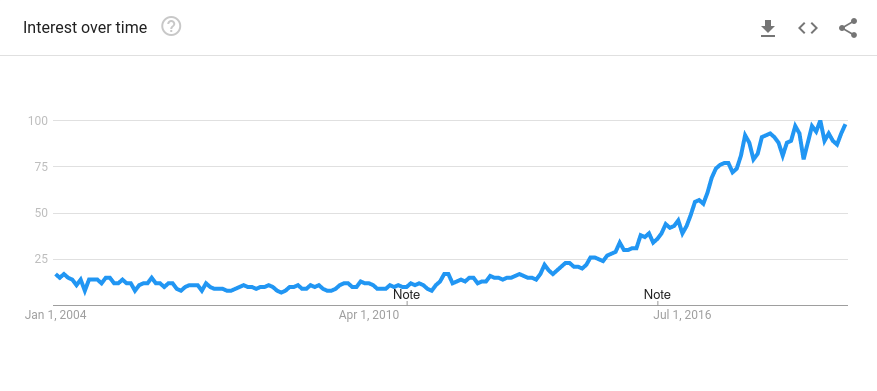
\includegraphics[scale=0.5]{./img/google-trends-ml.png}
            \captionsource{Machine Learning trends}{Google Trends}
            \label{fig:google-trends-ml}
        \end{center}
    \end{figure}

    \par Rozpowszechnienie Uczenia Maszynowego również spowodowało i moje zainteresowanie tematem.
    Z tego powodu dla swojej pracy licencjackiej wybrałem temat: Aplikacja uczenia maszynowego 
    metodą SVM.  Po zakończeniu pracy spodziewam się podwyższyć swoją kompetencje w dziale 
    Uczenia Maszynowego.

\subsection{Cel}
    \par Celem mojej pracy licencjackiej jest stworzenie oprogramowania pozwalającego na generowanie
    modeli używając Maszyny wektorów wspierających\textit{(ang. Support Vector Machine, SVM)} z graficznym 
    interfejsem użytkownika.  Program będą mogli użyć osoby potrzebujące szybko przetrenować kilka 
    modeli, przetestować ich dla różnych parametrów, zwizualizować dane. Program ma na celu ułatwienie
    pracę z Maszyną wektorów wspierających poprzez graficzny interfejs użytkownika
    oparty na bibliotekę QT. Część funkcjonalna programu jest oparta o bibliotekę LIBSVM\cite{CC01a}.

\subsection{Zakres}
    Program powinien móc ustawiać parametry dla wybranej metody oraz jądra\textit(ang. kernel), 
    generować wykresy podawanych zbiorów danych, interpretować różne formaty zbiorów danych, 
    wykonywać Sprawdzian krzyżowy (ang. Cross validation, CV), mieć metodę do optymalizacji 
    parametrów, pokazywać wyniki trenowania oraz testowania modeli.
\newpage

\section{Metoda klasyfikacji SVM} % SECTION
    \par W tym paragrafie w ogólnych zarysach jest opisana Maszyna Wektorów Wspierających
    oraz jej typy zaimplementowane w LIBSVM. Również będą krótkie opisy zaimplementowanych
    jąder.
\subsection{Opis}
    \par Swój program napisałem w oparciu o bibliotekę LIBSVM\cite{CC01a}. Maszyna Wektorów
    Wspierajacych(ang. Support Vector Machine. SVM) - klasyfikator, nauka którego ma na celu 
    wyznaczenie hiperpłaszczyzny rozdzielającej dwie klasy z maksymalnym marginesem. 
    Zaletą takiego klasyfikatora jest to że po uczeniu margines mówi jak dobrze są 
    odseparowane klasy. LIBSVM implementuje pięć typów Maszyny Wektorów Wspierajacych C-SVC, 
    $\nu$-SVC, One class SVM, $\epsilon$-SVR, $\nu$-SVR.
\subsection{C-SVC}
    \par C-Support Vector Classification - rodzaj klasyfikatora używający $C$ jako 
    parametr regularyzacji. Jeśli jest dany wektor $x_i \in R^n$, $i=1,...,l$ 
    w dwóch klasach i wektor etykiet $y_i \in \{1, -1\}$ to C-SVC rozwiązuję tak
    sformułowany problem:

    \begin{center}
        \begin{tabular}{rl}
            $\min\limits_{\pmb{\omega}, b, \varepsilon}$ & $\frac{1}{2} \pmb{\omega} ^T \pmb{\omega} +
            C \sum\limits_{i=1}^{l}\varepsilon_i$ \\
            Z zastrzeżeniem że & $y_i(\pmb{\omega}^T\phi(x_i) + b) \geq 1 - \varepsilon_i$ \\
                               & $\varepsilon_i \geq 0,i=1,...,l$
        \end{tabular}
    \end{center}

    \par Parametr $C$ służy do ustawienia marginesu: duży C $\rightarrow$ mały margines,
    mały C $\rightarrow$ duży margines.

    \begin{figure}[h]
        \begin{center}
            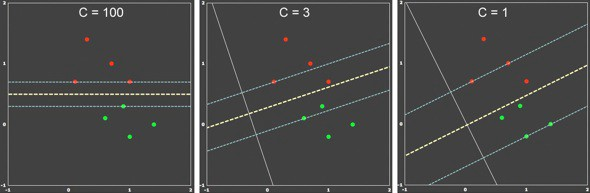
\includegraphics[scale=0.8]{./img/param_c.png}
            \captionsource{Zależność marginesu od parametru C}{\url{https://medium.com/@pushkarmandot}}
            \label{fig:param_c}
        \end{center}
    \end{figure}

    \par Dobry model dobrze separuję dane i razem z tym ma duży margines. Natomiast w
    w rzeczywistości jedno wyłącza drugie: duży margines włącza punkty z dwóch klas, a
    dobre separowanie może powodować przeuczanie(ang. Overfitting). Przeuczanie może 
    skutkować tym że model jest dobry na danych treningowych ale jest zły na danych testowych.

\newpage % description and equations was on different pages
\subsection{$\nu$-SVM}
    \par $\nu$-Support Vector Classification - rodzaj klasyfikatora używający $\nu$ jako
    parametr regularyzacji. Jest bardzo podobny do C-SVM, z różnicą że $\nu\in[0,1]$.
    Przyjemną właściwością $\nu$ jest to że on jest dolną granicą stosunku wektorów
    wspierających i górną granicą stosunku błędu uczenia.
    \par Jeśli jest dany wektor $x_i \in R^n$, $i=1,...,l$ w dwóch klasach i wektor
    $y\in R^l$ taki że $y_i \in \{1, -1\}$ to pierwotny problem optymalizacji wygląda
    następująco:

    \begin{center}
        \begin{tabular}{rl}
            $\min\limits_{\pmb{\omega},b,\varepsilon, \rho}$ &
            $\frac{1}{2}\pmb{\omega}^T\pmb{\omega} - \nu\rho + \frac{1}{l}\sum\limits_{i=1}^{l}
            \varepsilon_i$ \\
            Z zastrzeżeniem że & $y_i(\pmb{\omega}^T\phi(x_i) + b) \geq \rho - \varepsilon_i$ \\
                               & $\varepsilon_i \geq 0$, $i=1,...,l$, $\rho \geq 0$
        \end{tabular}
    \end{center}

\subsection{One-class SVM}
    \par One-class Support Vector Machine - rodzaj klasyfikatora uczenia
    nienadzorowanego, które zakłada brak etykiet w danych uczących. Ma na celu
    znalezienie niewiadomych wzorców/anomalii(klastrów) w danych wejściowych.  

    \begin{figure}[h]
        \begin{center}
            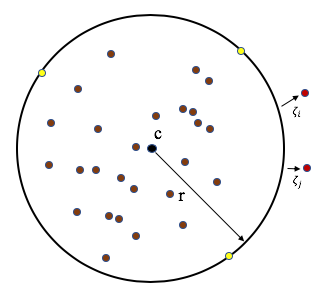
\includegraphics[scale=0.4]{./img/one-class-circle.png}
        \captionsource{Hipersfera zawierająca punkty danych. Ma środek c i promień R.
                        Punkty na krawędzi są wektorami wspierającymi.}{Wikipedia}
            \label{fig:param_c}
        \end{center}
    \end{figure}

    \par Jeśli dany jest wektor $x_i\in R^n$, $i=1,...,l$ bez informacji o klasach,
    to pierwotny problem optymalizacji wygląda następująco:

    \begin{center}
        \begin{tabular}{rl}
            $\min\limits_{\pmb{\omega},\varepsilon,\rho}$ & $\frac{1}{2}\pmb{\omega}^T\pmb{\omega} -
            \rho + \frac{1}{\nu l}\sum\limits_{i=1}^{l}\varepsilon_i$ \\
            Z zastrzeżeniem że & $\pmb{\omega}^T\phi(x_i)\geq\rho - \varepsilon_i$,\\
                               & $\varepsilon \geq 0$, $i=1,...,l$
        \end{tabular}
    \end{center}

\newpage
\subsection{$\epsilon$-SVR}
    \par Jeśli wektor etykiet $y_i \in R$ to jest używana metoda regresji.
    $\epsilon$-Support Vector Classification -  używa $C$ i $\epsilon$ jako
    parametrów regularyzacji. Celem jest znalezienie takiej funkcji $f(x)$
    że jej wartość odchyla się od $y_n$ na wartość nie większą od $\epsilon$
    dla każdego punktu z zbioru treningowego.
    \par Jeśli jest dany zbiór danych treningowych $\{(x_1, x_1),...,
    (x_l, z_l)\}$, gdzie $x-I \in R^n$ jest wektorem cech, a $z_i \in R^1$
    jest wyjściem. Przy danych parametrach $C>0$ i $\epsilon > 0$, standardowa 
    forma SVR to:

    \begin{center}
        \begin{tabular}{rl}
            $\min\limits_{\pmb{\omega},b,\pmb{\varepsilon}, \pmb{\varepsilon}^*}$ &
            $\frac{1}{2}\pmb{\omega}^T\pmb{\omega} + C\sum\limits_{i=1}^{l}
            \varepsilon_i + C\sum\limits_{i=1}^{l}\varepsilon_{i}^{*}$ \\
            Z zastrzeżeniem że & $\pmb{\omega}^T\phi(x_i) + b - z_i \leq \epsilon + \varepsilon_i$, \\
                           & $z_i - \pmb{\omega}^T\phi(x_i) - b \leq  \epsilon + \varepsilon_i^*$, \\
                           & $\varepsilon_i,\varepsilon_i^* \geq 0$,$i=1,...,l$

        \end{tabular}
    \end{center}

\subsection{$\nu$-SVR}
    \par $\nu$-Support Vector Regression - podobnie do $\nu$-SVC, używa parameter $\nu\in(0,1]$
    dla kontroli liczby wektorów wspierających. Również używa parametru $\epsilon$. Z parametrami
    $(C,\nu)$ $\nu$-SVR rozwiązuję:
    

    \begin{center}
        \begin{tabular}{rl}
            $\min\limits_{\pmb{\omega},b,\pmb{\epsilon},\pmb{\epsilon}^*,\epsilon}$ &
            $\frac{1}{2}\pmb{\omega}^T\pmb{\omega} + C(\nu\epsilon + \frac{1}{l}
            \sum\limits_{i=1}^{l}(\varepsilon_i+\varepsilon_i^*))$ \\
            Z zastrzeżeniem że & 
            $(\pmb{\omega}^T\phi(x_i) + b) - z_i \leq \epsilon + \varepsilon_i$,\\
           & $z_i - (\pmb{\omega}^T\phi(x_i) + b) \leq \epsilon + \varepsilon_i^*$,\\
           & $\varepsilon_i,\varepsilon_i^* \geq 0$, $i=1,...,l$, $\epsilon \geq 0$
        \end{tabular}
    \end{center}

\subsection{Jądra}
    \par 
\newpage
\section{Projekt aplikacji} % SECTION
\subsection{Opis}
\subsection{Technologie}
\newpage
\section{Podsumowanie} % SECTION
\subsection{Odniesienie do celu pracy}
\subsection{Co można dodać}

\newpage
\nocite{*}
\printbibliography

\end{document}
